% begin module transformations-absolute-value
\begin{frame}
What happens when we take the absolute value of a function?
\uncover<2->{
\[
|f(x)| = \left\{ \begin{array}{rcc}
f(x) & \textrm{if} & f(x) \geq 0\\
-f(x) & \textrm{if} & f(x) < 0
\end{array}\right.
\]
}
\uncover<3->{%
This tells us how to draw the graph of $y = |f(x)|$: the part of the graph above the $x$-axis remains the same; the part below the $x$-axis is reflected about the $x$-axis.
}
\uncover<4->{
\begin{example} %[Example 5, p. 41]
Draw the graph of the function $f(x) = |x^2 - 1|$.
\begin{columns}[c]
\column{.4\textwidth}
\psset{xunit=1cm, yunit=1cm}
\begin{pspicture}(-5, -5)(5,5) 
\psframe*[linecolor=white](-5,-5)(5,5) 
\psaxes[ticks=none, labels=none]{<->}(0,0)(-2.5,-1.5)(2.5,2.1)\tiny
\psLabelsWithOnes{2.5}{1.8}
\uncover<4>{
%Function formula: (x)^{2}-1 
\psplot[linecolor=red, plotpoints=1000]{-1.7}{1.7}{-1 x 2 exp add } 
}

\uncover<5->{
\psplot[linecolor=red, plotpoints=1000]{-1.7}{-1}{-1 x 2 exp add } 
\psplot[linecolor=red, plotpoints=1000]{1}{1.7}{-1 x 2 exp add } 
}

\uncover<5>{\psplot[linecolor=blue, plotpoints=1000]{-1}{1}{-1 x 2 exp add } }
\uncover<6->{
\psplot[linecolor=red, plotpoints=1000]{-1}{1}{x 2 exp -1 mul 1 add }
\rput[l](1.2,0.3){\alert<7>{$y=|x^{2}-1|$} }
}
\end{pspicture} 
%\ \only<handout:0| -4>{%
%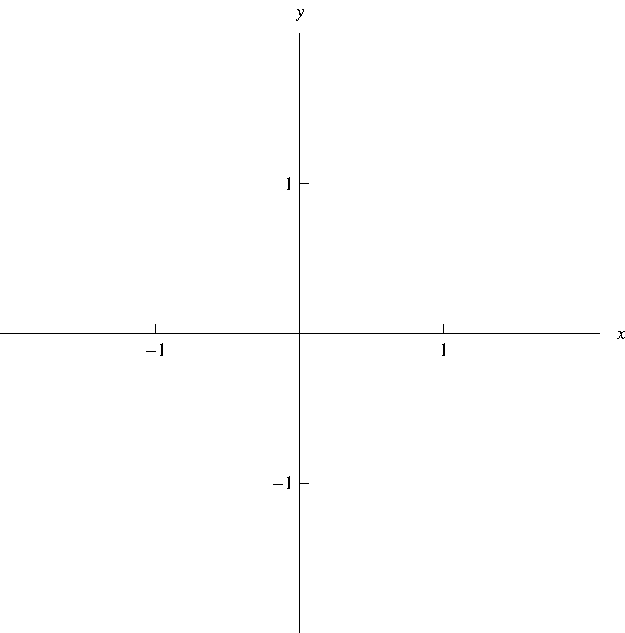
\includegraphics[height=4cm]{precalculus/pictures/01-03-ex5z.pdf}%
%}%
%\only<handout:0| 5>{%
%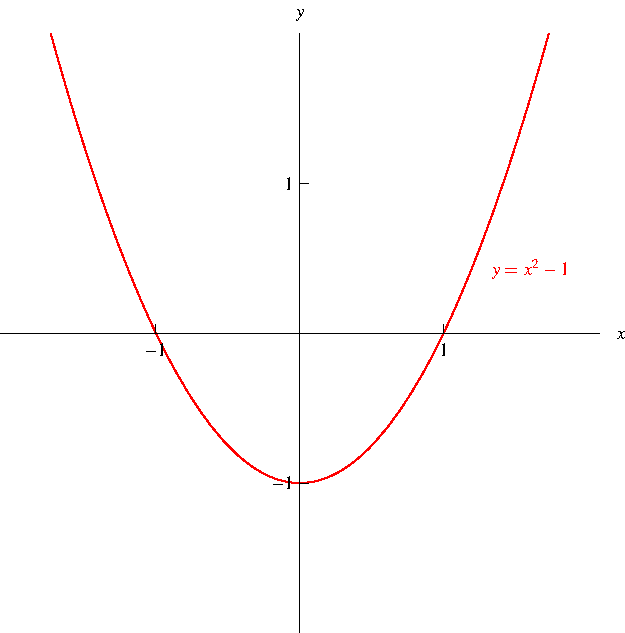
\includegraphics[height=4cm]{precalculus/pictures/01-03-ex5a.pdf}%
%}%
%\only<handout:0| 6>{%
%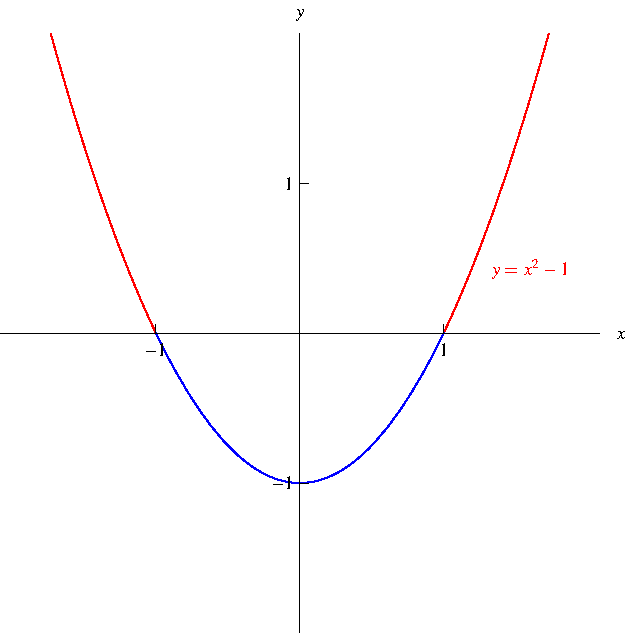
\includegraphics[height=4cm]{precalculus/pictures/01-03-ex5b.pdf}%
%}%
%\only<7->{%
%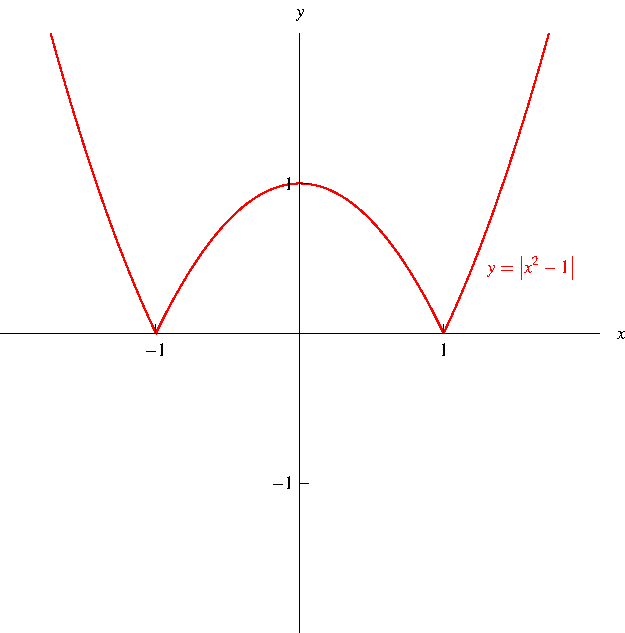
\includegraphics[height=4cm]{precalculus/pictures/01-03-ex5c.pdf}%
%}%
\column{.6\textwidth}
\begin{itemize}
\item<5->  Draw the graph of $f(x) = x^2 - 1$.
\item<6->  Identify the part(s) below the $x$-axis.
\item<7->  Flip those parts over the $x$-axis.
\end{itemize}
\end{columns}
\end{example}
}
\end{frame}
% end module transformations-absolute-value
